\section{Database View}

In this section is described the design of the database that will be used for the \textit{TrackMe} system. 

\begin{figure}[H]

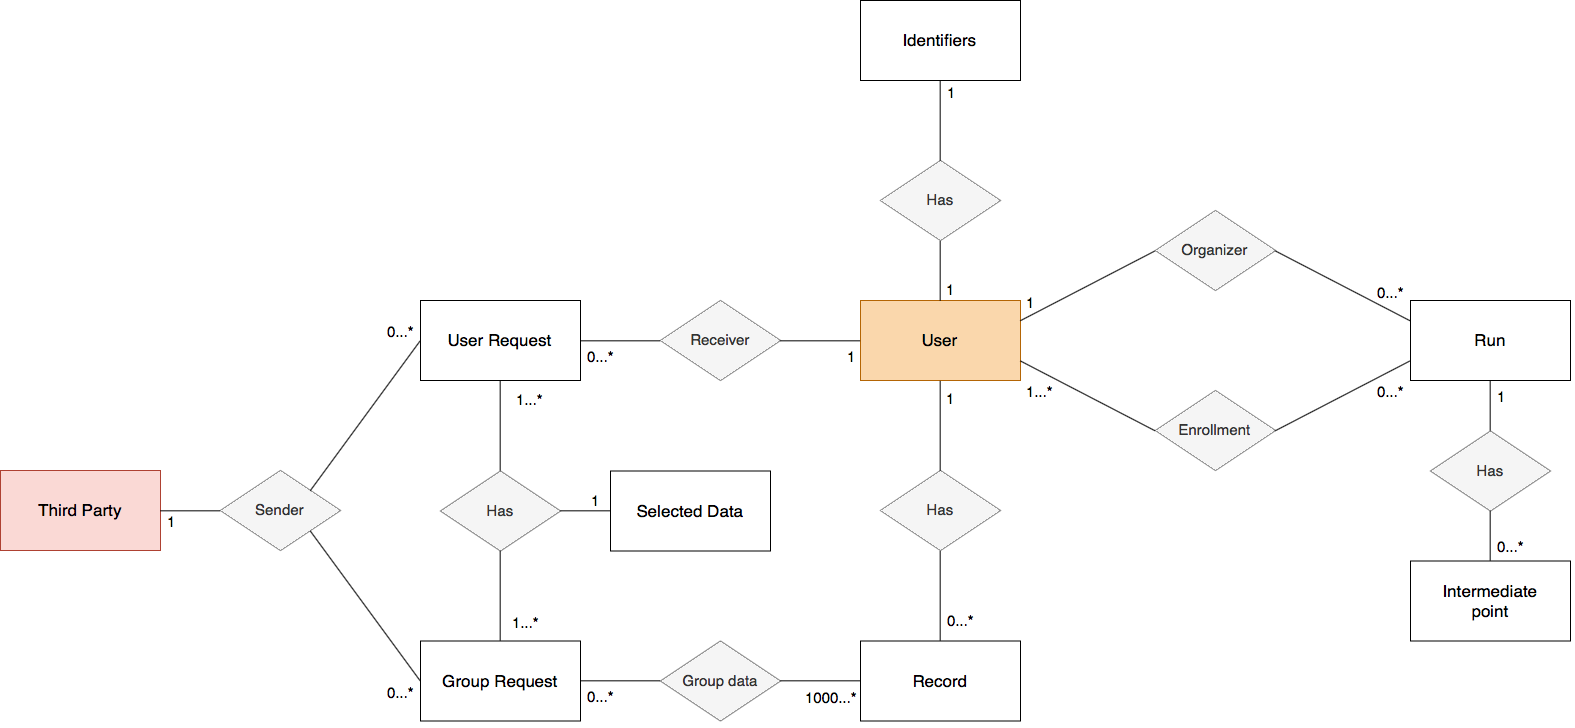
\includegraphics[scale=0.13,keepaspectratio]{./Pictures/ER-diagram.png}
\centering
\caption{Simplified ER diagram for the \textit{TrackMe} system}

\end{figure}

The picture above shows the main entities of the database. There is a \textit{User} entity, used to store the personal information of individual Users that is requested at sign up. Every User has many records associated to itself, each of them containing location and health data. This information is put in the \textit{Record} entity. The \textit{Third Party} entity contains meaningful data about the company that signed up to the \textit{TrackMe} system. Third Parties can make requests to the System in order to get access to User's data, so the \textit{Third Party} entity is related with the \textit{User Request} and the \textit{Group Request} entities. Both these entities contain information about the request, such as its status and the specific type of data to be accessed, but there is an important difference between the two regarding the anonymity of data. While a User request is sent to an individual User directly, a group request has a higher scope, and the data that is accessed after this type of request must be completely anonymous. The sender of the request must not get access to the personal data of the Users that have generated the records. To enforce this, the \textit{Group Request} entity is not related with \textit{User}, but instead directly with \textit{Record}. This solution is permitted by the use of anonymous identifiers, present in the \textit{Record} entity, that have a 1 to 1 relation with the Users of the system.

The \textit{Track4Run} service is represented by the Run entity, which has the information about the location, time and participants.

The \textit{AutomatedSOS} service does not rely on a complex data structure so it’s not displayed in the simplified ER diagram. Nevertheless, two attributes are present in the \textit{User} and \textit{Record} entities: the \textit{SosEnabled} attribute is a flag that indicates if the service is enabled or not; the \textit{isEmergency} attribute indicates if the record contains critical health parameters.

\begin{figure}[H]

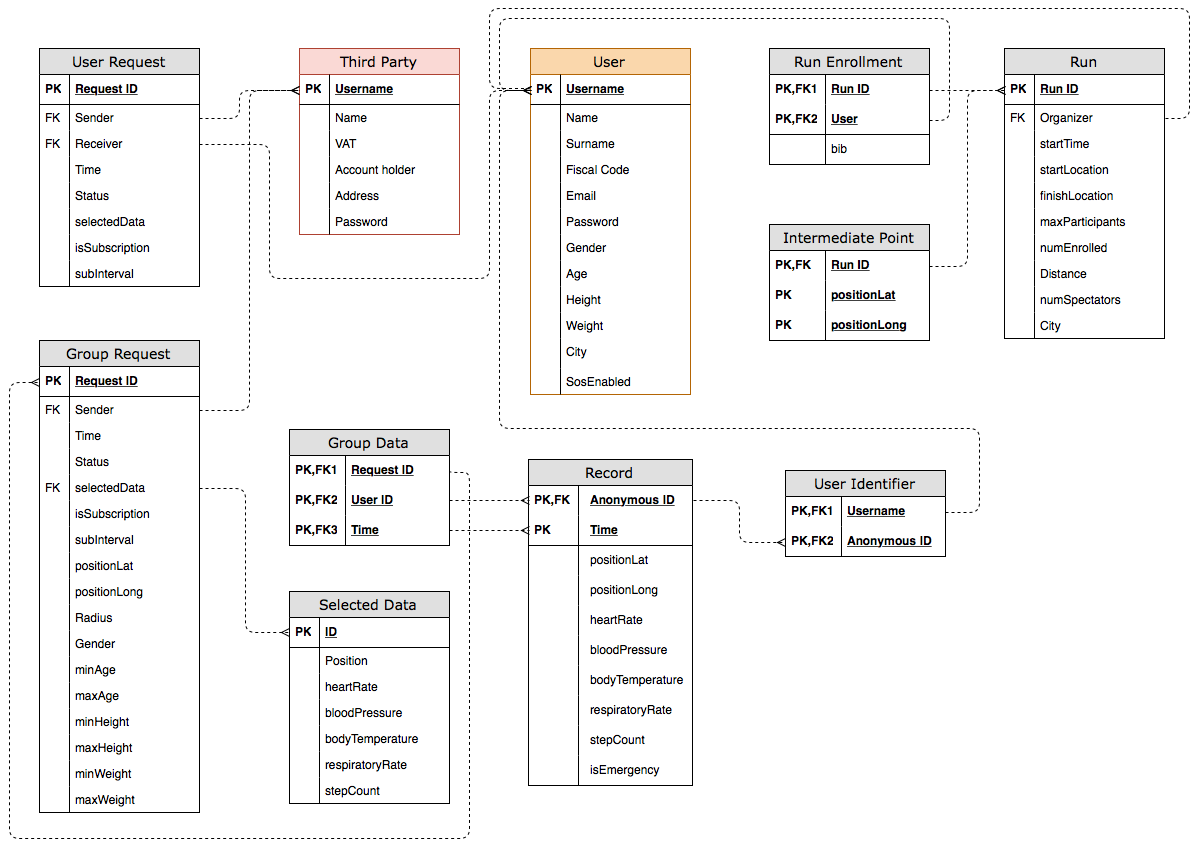
\includegraphics[scale=0.17,keepaspectratio]{./Pictures/ER-tables.png}
\centering
\caption{Tables and relative attributes of the \textit{TrackMe} database}

\end{figure}

Figure 2.9 represents a more complete representation of the \textit{TrackMe} database. Some of the attributes included in the diagram require some further explanation:

\begin{itemize}

\item[--] the \textit{Status} attribute of the \textit{User Request} table can take one of this three values: Accepted, Refused or Pending. As soon as the Third Party makes a request in the System, its \textit{Status} is set to Pending. When the User replies to the request it can either become Accepted or Refused, depending on the User's choice.
The \textit{Status} attribute is not present in the \textit{Group Request} because this type of request does not require User's interaction to be effective. In place of the \textit{Status} attribute, the \textit{isAllowed} attribute is used: it is a boolean that is defined automatically by the system after checking if the minimum number of 1000 interested Users is reached or not.

\item[--] the selection of the type of data to be accessed with a request is represented in the \textit{Selected Data} table. It contains 6 boolean values that indicate if the sender actually requests access to the specific type of data.
Given that a selection can be done in $2^6 = 64$ different ways, a unique integer identifier \textit{Selection ID} that ranges from 1 to 64 is put in place.

\item[--] the attributes in the \textit{Record} table represent all the types of data supported by the system. Users’ smart devices may not be equipped with the sensors needed to acquire certain type of data (for example, smart sensors for respiratory rate monitoring are not easily available in the market), so instances of this entity do not have to contain all of them. To signal the absence of data, a special value is stored. 

\item[--] the \textit{subInterval} attribute in the \textit{User Request} and \textit{Group Request} tables indicates the time between two data updates in a subscription request. It is therefore used only if the \textit{isSubscription} attribute contains the value True and it can take 4 different values: hour, day, week or month. 

\end{itemize}